% Этот текст можно свободно редактировать.
\FloatBarrier
\section{GPT-2 и честное сравнение}

GPT2LMHeadModel обучен с нуля: 2 causal decoder layers, 4 attention heads, width 128 (выбор из 96/128 по validation NDCG@10), tied input/output embeddings. Токен --- ID трека. Dropout .1 при SFT; AdamW lr .001, batch 32, до 8 эпох, patience 2, clip gradient norm 1.

В SFT выбраны 30 000 перекрывающихся окон (stride 32) из train. Всего 645,171 допустимых target positions на эпоху с учётом повторов в окнах. Loss --- next-token CE только для известных, неорганических и однозначных по времени целей. Органические события и UNK входят в контекст. У коротких историй BOS и левый padding; loss на padding отсутствует.

SFT checkpoint выбирается по validation. Для выбранной архитектуры обучены отдельные seed 42/43/44. Все варианты дообучения внутри seed стартуют с одной и той же сохранённой SFT. Continued-CE получает те же 300 updates и те же начальные префиксы. Его set loss
\begin{equation}
\mathcal L_{\mathrm{CE}}=-\log\sum_{i\in P_t}\pi_\theta(i\mid s_t),
\end{equation}
где \(P_t\) --- известные неорганические цели timestamp-группы; при одной цели это обычный CE. Тот же loss используется в balanced auxiliary term. Это контроль дополнительного обучения; число FLOPs, actions и затраты времени не приравниваются.

Оценочный запрос --- user/timestamp с неорганическими событиями; положительные объекты --- уникальные неорганические item ID этой группы. Ранжирование точное по всем 16 384 доступным трекам, без sampled negatives. Повторы разрешены: в музыке знакомый трек может быть релевантен. Поэтому repeat --- диагностика, а не автоматически ошибка.

Оценочные запросы равномерно сэмплируются без возвращения из всех подходящих timestamp-групп: 512/1024/2048 на validation/confirmation/test. Для 12 000 RL/continued-CE train states дополнительно требуется хотя бы одна known positive, чтобы определить CE loss. Во временных holdout такого фильтра нет; полностью OOV-запросы сохраняются. Для всех методов используются одни и те же cached queries.

В test 2048 запросов у 434 пользователей; 931 запросов полностью вне словаря. Общие Recall/NDCG/MAP@5/10/20 включают OOV-цели с нулевым вкладом. Conditional-метрики делят только на известные цели и исключают полностью OOV-запросы. Это разные estimands.

Query-macro NDCG использует бинарную релевантность, ideal DCG по min(K, число всех целей); MAP --- сумму precision на hit-позициях, делённую на min(K, число целей). Для conditional вариантов знаменатели пересчитываются по known targets. Дополнительные контроли: train popularity и \(0.9\cdot\text{частота в текущем контексте}+0.1\cdot\text{train popularity}\).

Позитивом считается любой logged неорганический listen, включая малый completion. Поэтому ranking metrics измеряют matching исторических действий logging policy, а не экспертную или причинную удовлетворённость. Снижение NDCG само по себе не доказывает ухудшение пользовательского опыта; концентрация и другие диагностики помогают понять характер изменения.

\begin{figure}[!htbp]
\centering
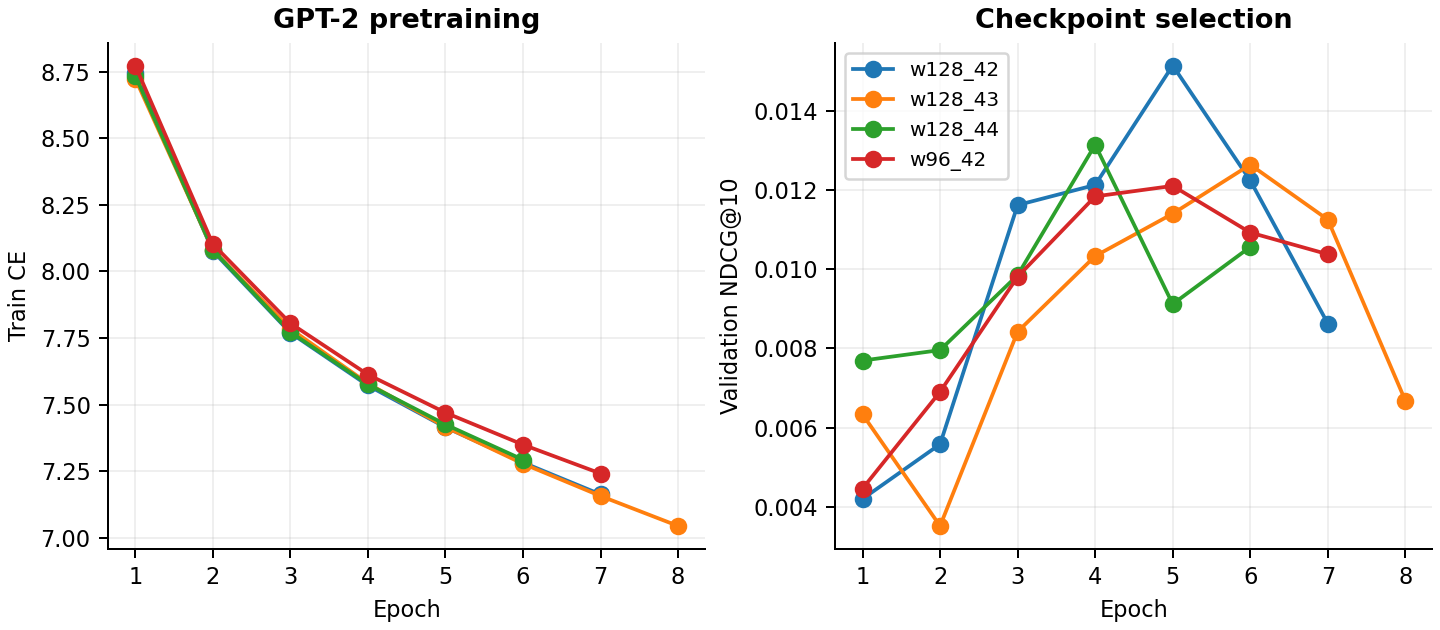
\includegraphics[width=\linewidth,height=.70\textheight,keepaspectratio]{figures/sft_curves.png}
\caption{Обучение и выбор SFT checkpoint; test не используется для остановки.}
\label{fig:sft-curves}
\end{figure}
